\documentclass[bigger]{beamer}

\usepackage{czech}
\usepackage[utf8]{inputenc}
\usepackage{booktabs}
\useinnertheme{rounded}
\usecolortheme{crane}
\setbeamerfont{block title}{size={}}

\newcommand{\img}[2]{\begin{center}\includegraphics[width=#1\linewidth]{#2}\end{center}}

\title{Adaptive Learning\\Ukázky vyvinutých systémů a analýz}

\author{Radek Pelánek\\[10mm]
  
\includegraphics[width=.2\linewidth]{al-logo-researchgroup}}

\date{2017}

\begin{document}

\frame{\titlepage}

\begin{frame}
  \frametitle{Ukázky systémů}

  \begin{itemize}
  \item \textbf{Slepé mapy} (další podobné: Anatom, Poznávačka přírody)
  \item \textbf{Umíme česky} (další podobné: Umíme anglicky, Umíme matiku)
  \item \textbf{Robomise}
  \end{itemize}
\end{frame}

\begin{frame}
  \frametitle{Slepé mapy}

  \texttt{slepemapy.cz}

  \bigskip

  \begin{itemize}
  \item dostupný obsah
  \item podoba otázek
  \end{itemize}
\end{frame}

\begin{frame}
  \frametitle{Slepé mapy: AB experimenty}

  \begin{itemize}
  \item náhodný X adaptabilní výběr otázky
  \item cílová obtížnost otázek: 50 \%, 65 \%, 80 \%, 95 \%
  \item počet distraktorů: od 2 do 6
  \item způsob volby distraktorů
  \end{itemize}  
\end{frame}

\begin{frame}
  \frametitle{Slepé mapy: hodnocení obtížnosti otázek}

  \img{.95}{ratings}
\end{frame}

\begin{frame}
  \frametitle{Umíme česky}

  \texttt{umimecesky.cz}

  \bigskip

  \begin{itemize}
  \item strom konceptů, mapa učiva
  \item míra znalostí, \uv{mastery learning}
  \item netradiční hry: Střílečka, Tetris, hry pro více hráčů
  \end{itemize}
\end{frame}

\begin{frame}
  \frametitle{Robomise}

  \texttt{robomise.cz}

  \bigskip

  \begin{itemize}
  \item kontext: Hour of code
  \item základní prostředí postavené na Blockly
  \item inovativní pojetí úlohy
  \item adaptivní chování
  \end{itemize}
\end{frame}

% \begin{frame}
%   \frametitle{Ukázky analýz}

%   \begin{itemize}
%   \item podobnost položek
%   \item křivky přežití, křivky učení
%   \item vyhodnocení kritérií zvládnutí
%   \end{itemize}
% \end{frame}

\begin{frame}
  \frametitle{Analýza obtížnosti}

  \img{.5}{mult_dif}
\end{frame}

\begin{frame}
  \frametitle{Časté chyby}

  \img{.75}{mult_mistakes}
\end{frame}

\begin{frame}
  \frametitle{Časté chyby}

  \img{1}{analyza-carky}
\end{frame}

\begin{frame}
  \frametitle{Podobnost položek: co si lidé pletou}

  \img{.8}{confusion-clustering-map}
\end{frame}

\begin{frame}
  \frametitle{Podobnost položek: projekce do roviny}

  \img{1}{vyjmslovab}
\end{frame}

\begin{frame}
  \frametitle{Vyhodnocení kritérií zvládnutí}

  \begin{center}
    \begin{tabular}{ccc}
      simulovaná data & & reálná data \\
      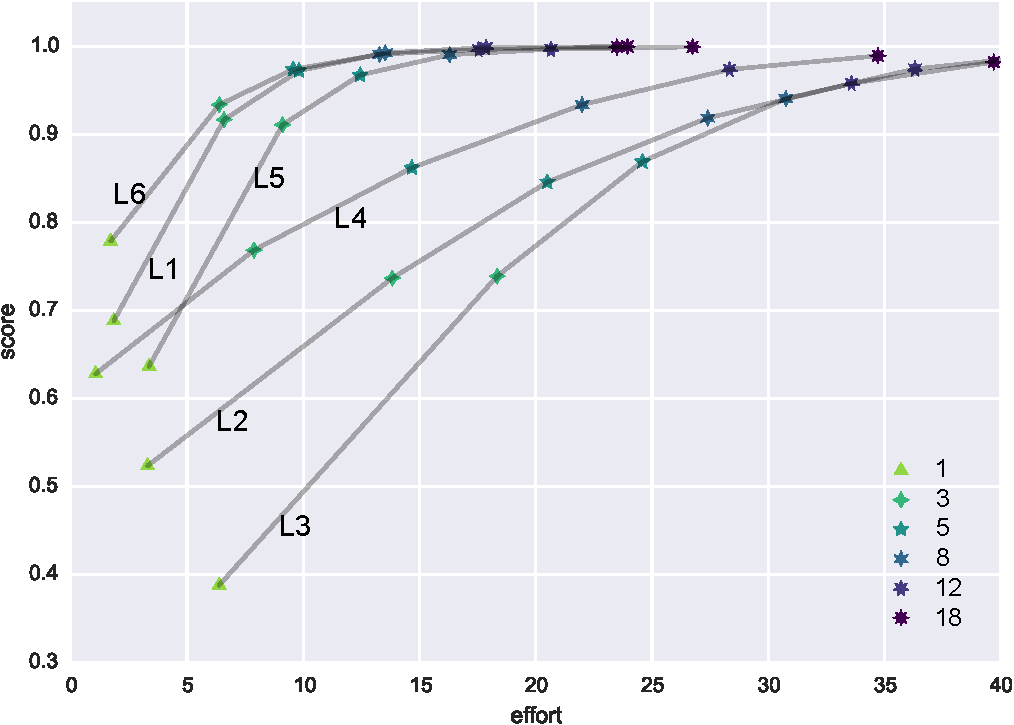
\includegraphics[width=.45\linewidth]{ncc-effort-score} & &
      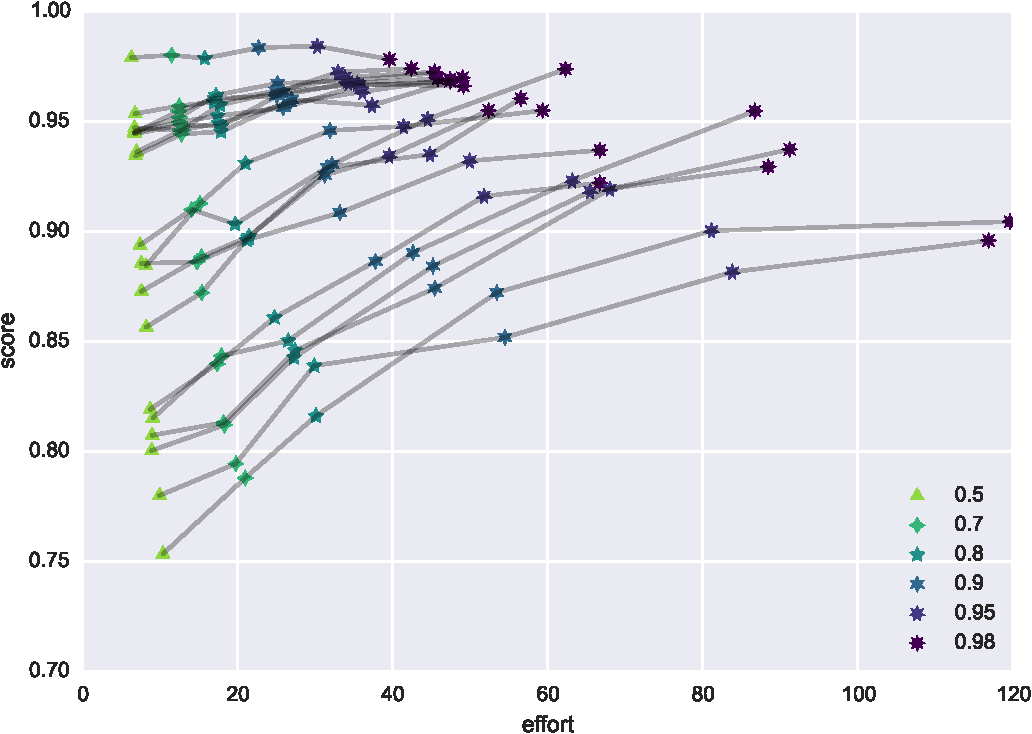
\includegraphics[width=.45\linewidth]{uc-effort-score}
    \end{tabular}
  \end{center}
\end{frame}

\begin{frame}
  \frametitle{Adaptive Learning}

  \begin{itemize}
  \item praktický vývoj výukových systémů
  \item analýzy dat
  \item evaluace, obecné metodické otázky
  \end{itemize}
\end{frame}

\end{document}